\chapter{Results and Discussion}
\label{chap:results}

\section{Testing Environment}
\label{sec:test_env}

The model was evaluated on the following hardware:
\begin{itemize}
    \item \textbf{Mobile Phone:} iPhone 13 (A15 processor).
    \item \textbf{Laptop:} Macbook Pro 2018 (Intel Core i7 processor).
    \item \textbf{Cloud Environment:} Google Colab (Tesla T4 GPU).
\end{itemize}

\section{Quantitative Evaluation}
\label{sec:quantitative_eval}

The final student model's performance was evaluated on a test set from NYU Depth V2 consisting of 400 images, and it was compared against the teacher model.
The Table~\ref{tab:quantitative_results} shows the achieved results using the metrics defined previously in Section~\ref{sec:evaluation_metrics}.

\begin{table}[htbp!]
    \centering
    \caption{Quantitative Evaluation of the Student Model.}
    \label{tab:quantitative_results}
    \resizebox{\textwidth}{!}{%
        \begin{tabular}{lccccccc}
            \toprule
            \textbf{Model} & \textbf{Abs Rel ($\downarrow$)} & \textbf{Sq Rel ($\downarrow$)} & \textbf{RMSE ($\downarrow$)} & \textbf{RMSE Log ($\downarrow$)} & \textbf{$\delta < 1.25$ ($\uparrow$)} & \textbf{$\delta < 1.25^2$ ($\uparrow$)} & \textbf{$\delta < 1.25^3$ ($\uparrow$)} \\
            \midrule
            Teacher & 0.2853 & 0.6857 & 1.4286 & 0.3273 & 0.6236 & 0.8340 & 0.9247 \\
            Student & 0.4068 & 0.9911 & 1.6713 & 0.3877 & 0.5733 & 0.8261 & 0.8911 \\
            \bottomrule
        \end{tabular}%
    }
\end{table}

\section{Qualitative Evaluation}
\label{sec:qualitative_eval}

The model was tested on various images. The Figure~\ref{fig:qualitative_comp} shows a comparison between the original image (left), the depth map from the teacher (middle), and the depth map from the student (right).

\begin{figure}[htbp!]
    \centering
    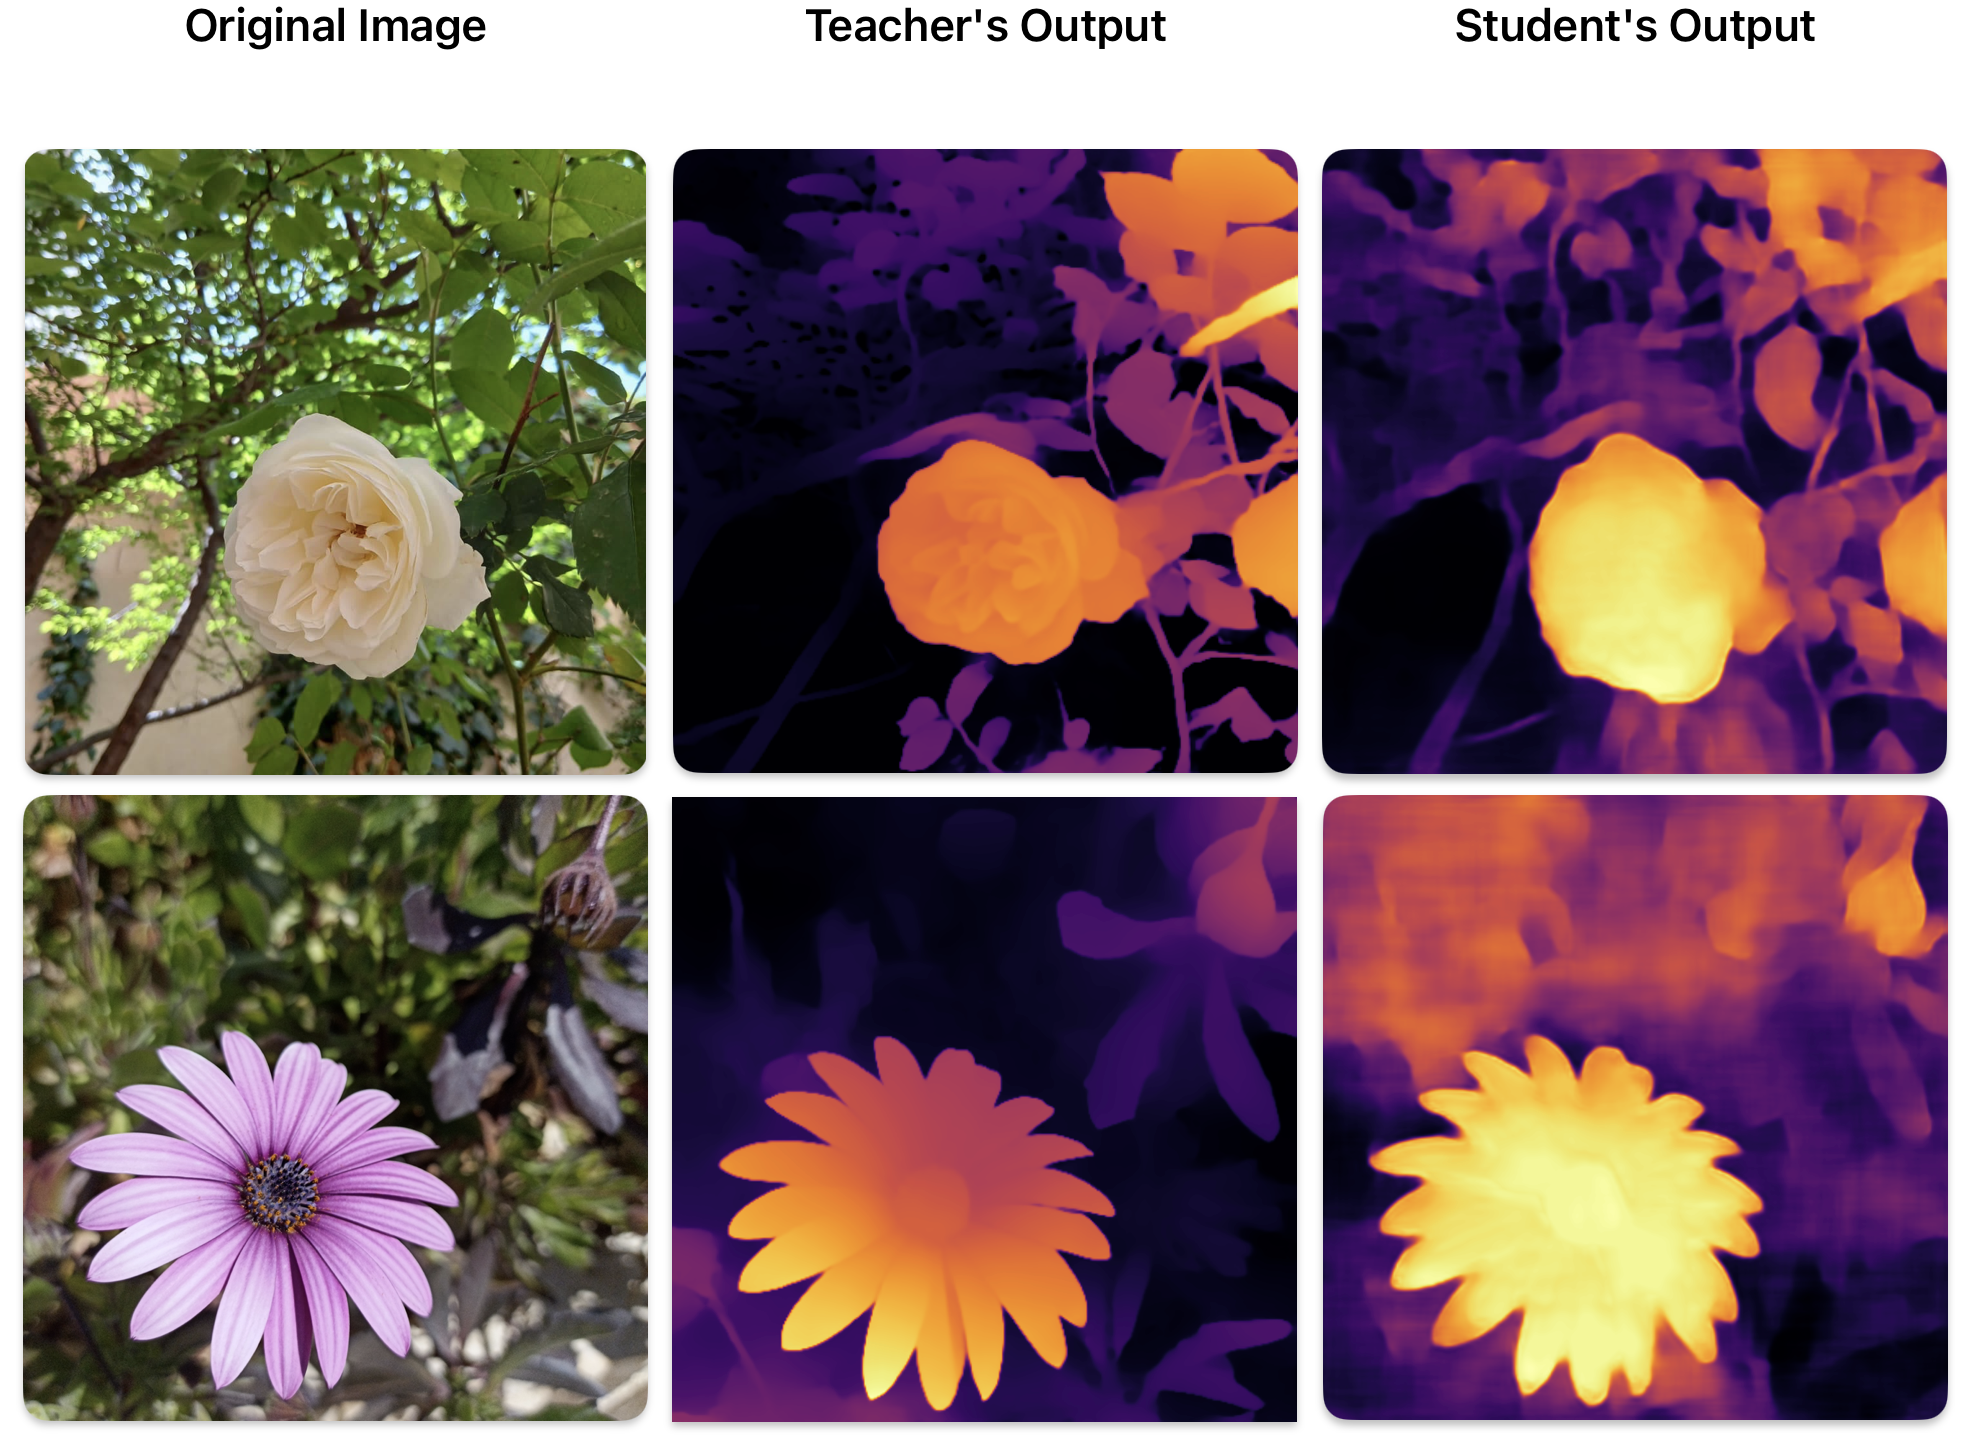
\includegraphics[width=\textwidth]{images/qualitative_comparison.png}
    \caption{Visual Comparison.}
    \label{fig:qualitative_comp}
\end{figure}

\section{Performance Measurements}
\label{sec:performance}

Performance was measured on the devices mentioned in the testing environment, and the results were as shown in Table~\ref{tab:performance}.

\begin{table}[htbp!]
    \centering
    \caption{Performance Measurements for the Model.}
    \label{tab:performance}
    \begin{tabular}{lc}
        \toprule
        \textbf{Model} & \textbf{Time (milliseconds)} \\
        \midrule
        Teacher on Laptop & $1124 \pm 10$ \\
        Student on Laptop & $576.8 \pm 10$ \\
        Teacher on Google Colab & $60 \pm 7$ \\
        Student on Google Colab & $13.2 \pm 3$ \\
        Teacher on Mobile Phone & $10751 \pm 50$ \\
        Student on Mobile Phone & $186 \pm 10$ \\
        \bottomrule
    \end{tabular}
\end{table}

We achieved an average time of 186 milliseconds on the mobile phone, which means we have achieved the desired goal.

\section{Discussion}
\label{sec:discussion}

This project has succeeded in achieving its primary objective: to demonstrate the effectiveness of knowledge distillation as a strategy for developing highly efficient depth estimation models suitable for mobile devices. The results show that the developed student model is capable of operating in near real-time within a resource-constrained environment, thus achieving the difficult balance between computational accuracy and performance requirements. Achieving an average inference time of about 186 milliseconds on a mobile phone meets the non-functional requirement of not exceeding 200 milliseconds and confirms the success of the adopted approach.

When analyzing the results, we note an expected gap in accuracy between the teacher and student models, as shown by the quantitative evaluation on the NYU Depth V2 dataset. It is worth noting that the performance of the teacher model, according to its developers, is better than what was measured here (0.05 for AbsRel~\cite{yang2024depthV2}), which indicates a bias in the dataset used for evaluation. Therefore, we focus on the gap between the student and teacher rather than the absolute value of the metrics. While this accuracy gap makes the model unsuitable for applications requiring high precision, it is well-suited for fields that tolerate a larger margin of error, such as navigation assistance. This decrease in accuracy represents a deliberate and acceptable trade-off in exchange for obtaining massive gains in performance.

The model size was reduced by a ratio of approximately 1/7 compared to the teacher. More importantly, it is now possible to run it on a mobile device with near real-time performance, which was not possible with the teacher model. Qualitative comparisons show that the student model successfully captures the general structure of the scene and the fundamental depth gradients, despite losing some of the fine details that the teacher model retains. This quality is considered sufficient for many practical applications, such as augmented reality and basic navigation aids.

The success of the model can be attributed to several deliberate methodological decisions. The choice of the MobileViT-XS architecture as the encoder was a crucial decision, as it proved its ability to understand the global context of the image, overcoming the limitations of the MobileNetV3 architecture observed in initial attempts. Furthermore, the composite loss function played a pivotal role in the distillation process: by compelling the student to mimic not only the final output but also the teacher's intermediate gradients and feature maps, a more comprehensive set of knowledge was transferred, which helped maintain the quality of the results despite the model's smaller size.

However, the project is not without limitations. Challenges that could be addressed in future work include improving depth estimation for transparent or reflective surfaces, which are known to be difficult for monocular depth models. Additionally, the model's performance in low-light conditions could be addressed by performing image pre-processing (e.g., increasing contrast).

\section{Future Work}
\label{sec:future_work}

Based on this discussion, several promising avenues for future work can be identified:
\begin{itemize}
    \item \textbf{Improve Training Data:} The most important next step is to retrain the model on more diverse public datasets like NYU Depth V2 to enhance its generalization capabilities and reduce the impact of biases in the current data.
    \item \textbf{Improve Evaluation Data:} To obtain logical and fair values for the metrics mentioned in the reference study.
    \item \textbf{Multi-stage Distillation:} This involves training a model with a number of parameters closer to the teacher (e.g., 15 million), then using it as a teacher for a smaller model, and finally using the latter as a teacher for the student model designed in this project.
    \item \textbf{Additional Architectural Improvements:} Other hybrid architectures could be explored, or the MiniDPT decoder structure could be improved to reduce the accuracy gap with the teacher without a significant increase in computational cost.
    \item \textbf{Model Quantization:} As a final optimization step, quantization techniques (such as converting weights to 16-bit or 8-bit integers) can be applied to the final ONNX model. This procedure would further reduce the model's size and accelerate inference time on supported mobile devices.
\end{itemize}